\chapter{Methodology}
\label{chap:metodologia}

In this chapter, we present the research methodology which is composed of three steps: the literature review, the Grounded Theory. Section \ref{sec:methodology-overview} gives an overview of the research methodology. Section \ref{sec:methodology-slr} explains the Systematic Literature Review process. Section \ref{sec:methodology-gt} shows how the Grounded Theory method was applied.


\section{Overview}
\label{sec:methodology-overview}
The methodology consists of three steps: \textit{State-of-the-Art}, \textit{Qualitative Analysis}, and the \textit{Guidelines} formulation. The Systematic Literature Review of the State-of-the-Art step aims to review the existing evidence concerning the impact evaluation of multimodal interfaces and seeks to summarize the empirical evidence concerning the strengths and limitations of a specific evaluation method \cite{Kitchenham2007}. In Qualitative Analysis, the Grounded Theory \citeonline{Glaser1967} builds a theory of cognitive impact evaluation from data retrieved in the Systematic Literature Review. After, we offer guidelines based on all data analyzed and the discussion of weak points encountered of cognitive impact evaluation of multimodal interfaces for people who are blind or visually impaired. 


\section{Systematic Literature Review}
\label{sec:methodology-slr}
In contrast to an ad-hoc literature review, the systematic literature review is a methodologically rigorous analysis and study of research results. To achieve our goal, the main research question for this first part of the proposal was \textbf{``How is the cognitive impact evaluated on multimodal interfaces for people who are blind''}. For a better understanding, as a second goal question, we aim to learn the challenges regarding impact evaluation on this scenario.

The process of a systematic literature review includes three main phases: planning the review; conducting the review and reporting the review \cite{Kitchenham2007}. During all process of the systematic literature review, we used the tool StArt (``StArt'', 2016) and the software Microsoft Excel\footnote{Microsoft Excel - \url{https://products.office.com/pt-br/excel}} as a support to create the protocol, apply the filters, select the papers and show the results. We organize all references on software Mendeley\footnote{Mendeley - \url{https://www.mendeley.com/}}. As the papers retrieved from PubMed Central are in MEDLINE format, we developed the tool Medline2bibtex\footnote{Medline2Bibtex - \url{https://github.com/lanabia/Medline2Bibtex}}. It works as a parser to permit the list to be read by both StArt and Mendeley.

Each of these stages has a qualitative methodological design that aims to offer a better specification and evolution in the development of the systematic literature review. Figure \ref{fig:systematic_literature_review} presents the SLR process adopted in this study by using a UML language\footnote{UML - \url{http://www.uml.org/}} for Activity Diagram. The process suits the guidelines from \cite{Kitchenham2007}. The next subsections describe the planning (the study selection criteria, the research sources selected) and the conducting phase (the search Process, the data extraction form fields and the studies quality evaluation). The entire process was stored in an excel worksheet available online\footnote{\url{https://www.dropbox.com/s/dvvn44cymqsqguy/Systematic\%20Review\%20-\%20Mesquita\%20L.\%202018.xlsm?dl=0}}.

 	\begin{figure}[h] 
   	    \captionsetup{width=16cm}%Da mesma largura que a figura
		\Caption{\label{fig:systematic_literature_review} Systematic Literature Review Process}
		\UFCfig{}{
			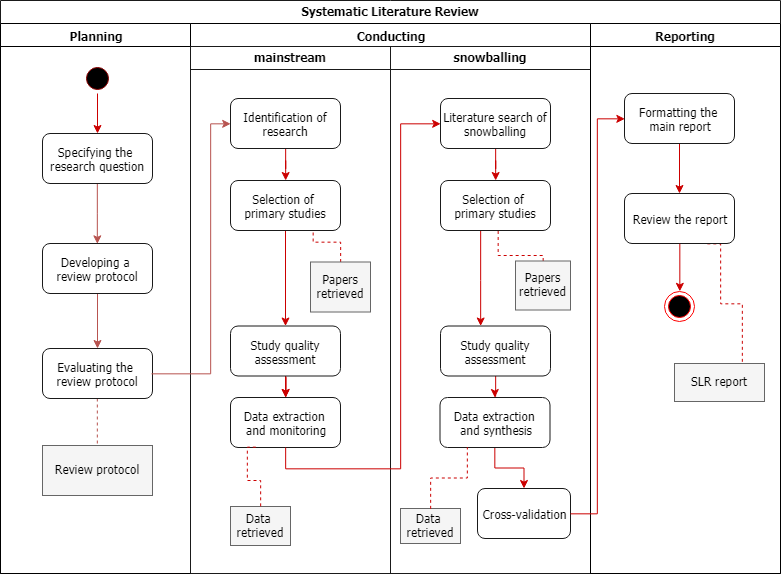
\includegraphics[width=16cm]{figuras/systematic_literature_review.png}
		}{
			\Fonte{Produced by the author based on \citeonline{FACANHA2018}.}
		}	
	\end{figure}

\subsection{Planning: definition of the protocol}
\label{subsec:methodology-planning}

In the planning phase, we define a review protocol that specifies the research question being addressed and the methods that will be used to perform the review \cite{Kitchenham2007}. The overall goal of this systematic literature review is to analyze the state-of-the-art and the study opportunities related to the cognitive impact evaluation of multimodal interfaces for people who are blind. Then, we addressed the following main and second questions.

    \begin{itemize}
        \item \textbf{Main question}: How is the cognitive impact evaluated on multimodal interfaces for people who are blind?

        \item \textbf{Second question}: Which are the challenges regarding impact evaluation on this scenario?
    \end{itemize}
    
\textbf{Sources selection}

The first suggested digital libraries as sources are: \textit{ACM Digital Library}; \textit{Engineering Village}; \textit{IEEE Xplore}; \textit{Scopus}; \textit{Science Direct}; \textit{Springer Link}; \textit{PubMed}; \textit{Web of Science}; \textit{Google Scholar}, that includes the leading conferences and journals from Computer Science.

The bases chosen are the primary research bases for scientific articles in the research area or the bases that index them. Since Scopus, which index ACM Digital Library and IEEE Xplore, is based on the same database of ScienceDirect. So, we choose Scopus that is considered the most effective search engine \cite{Burnham2006}. 

We withdrew Engineering Village because their twelve engineering document databases covered do not cover the content of this research. Scopus and Web of Science do not have the same database \cite{Tober2011}, so we maintain these two in the final source list. As the research include visual disabilities, we expect to find some works in PubMed database.

Although Google Scholar is declared as a credible alternative at the same level of Scopus in the face of the Web of Science \cite{Harzing2016}, it is not considered as a database, and it is only considered as a search engine. The final list of sources to systematic literature review is \textit{Scopus}, \textit{Springer}, \textit{Web of Science} and \textit{PubMed Central}.

We also research in the Journal of Visual Impairment \& Blindness that addresses a variety of topics related to visual impairment. The research in this journal changes a little the string applied to get their proceedings, that are in the scientific base PubMed Central.

\textbf{Studies initial selection}

The initial selection occurs by applying a search string into in each source. Before the final version of the string, we simulated many other strings in searching the best solution and results with the principal papers of the area, covering a broad range of possible papers in the search criteria. The final string defined was the string bellow.

The string will be applied on the metadata of papers, that includes abstract, index terms, and bibliographic citation data (such as document title, publication title, etc.). The research in the sources are applied by using the research string and the two initial criteria: to be published after 1998 and to be written in English. Based on the goal of systematic literature review we define the search string as shown in the Figure \ref{fig:string}.

 	\begin{figure}[h] 
   	    \captionsetup{width=14cm}%Da mesma largura que a figura
		\Caption{\label{fig:string} Search string}
		\UFCfig{}{
			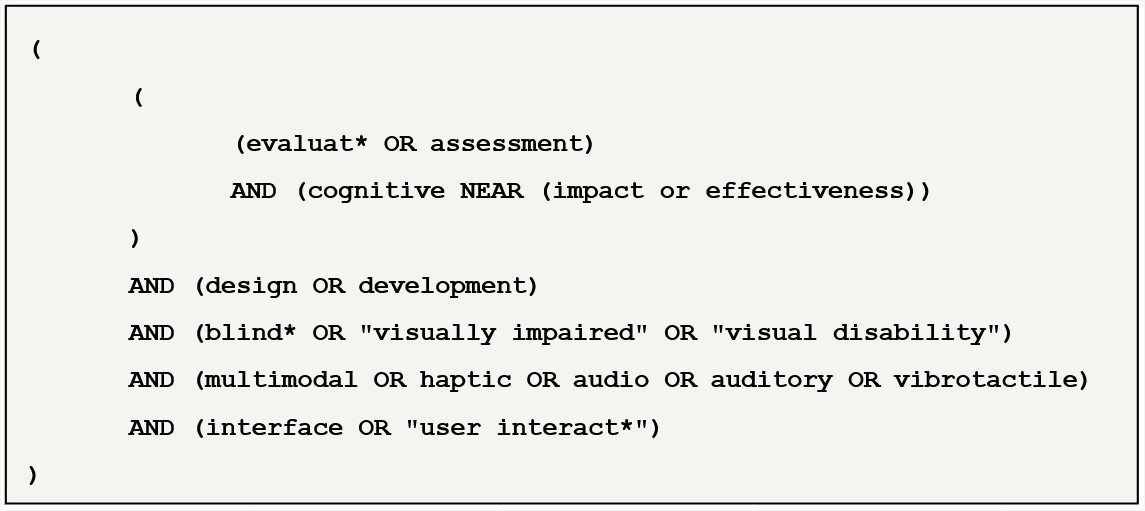
\includegraphics[width=14cm]{figuras/string.jpg}
		}{
			\Fonte{Produced by the author.}
		}	
	\end{figure}

%%Nao ficou legal em código, mas deixei ai caso vc queira testar%%
%\begin{lstlisting}[]
%(
%    (
%     (evaluat* OR assessment)
%     AND ((cognitive OR psychomotor OR physical OR emotional)
%                (NEAR/10 (impact or effectiveness))
%    )
%    AND (design OR development)
%    AND (blind* OR "visually impaired" OR "visial disability")
%    AND (multimodal OR hapatic OR audio OR auditory OR vibrotactile)
%    AND interface
%)
%\end{lstlisting}

\textbf{Study selection criteria}

We define the search criteria as studies that present technology for people who are blind or visually impaired and has applied a cognitive impact evaluation. The inclusion and exclusion criteria are according to the goal of the systematic literature review. These requirements comply the general objective of this study, but also aim to have a broader view of the assessment in various technologies in the area. Table \ref{tab:inclusion_and_exclusion_criteria} presents the inclusion \textit{(I)} and exclusion \textit{(E)} selection criteria. To be accepted, a scientific paper must cover all inclusion criteria and none exclusion criterion.

\begin{table}[h]
	\captionsetup{width=16cm}%Deixe da mesma largura que a tabela
	\Caption{\label{tab:inclusion_and_exclusion_criteria} Inclusion and exclusion criteria}%
	\IBGEtab{}{%
		\begin{tabular}{m{1cm}m{6cm}m{1cm}m{6cm}}
			\toprule
			Code & Inclusion Criteria & Code & Exclusion Criteria \\
			\midrule \midrule
			I.01 & The study has the technology for people who are blind or visually impaired & E.01 & Title and abstract out the search criteria (I.02, I.03, I.04) \\
			I.02 & The study evaluates the technology by using some approach that involves the user & E.02 & Entire text out the search criteria (I.02, I.03, I.04) \\
			I.03 & The study evaluates the technology by using a method to evaluate the cognitive impact & E.03 & The document is a book, a congress’ abstract, an extended abstract, a poster, an oral communication, proceedings of a conference, a seminar, a research plenary, a dictionary or an encyclopedia \\
			 & & E.04 & The study must be published after 1998 and written in English \\
			\bottomrule
		\end{tabular}%
	}{%
	\Fonte{Produced by the author.}%
%	\Nota{esta é uma nota, que diz que os dados são baseados na	regressão linear.}%
%	\Nota[Anotações]{uma anotação adicional, seguida de várias outras.}%
    }
    \end{table}

The technologies defined in the \textit{I.01} criterion include mobile application, computer software, IoT systems, virtual environments or a video game with multimodal interfaces. Also, we accept technologies that are not specifically for people who are blind or visually impaired with the goal of expanding the results, but the studies present the technology focused on users with visual disabilities. We exclude from all technologies that uses Sensory Substitution Devices \cite{Pissaloux2017TowardsDevices}, which substitutes a sense. The device SSD (Sensory Substitution Devices), out of our scope, includes sensory replacement, haptics as sensory augmentation, bionic eyes, retinal visual prosthesis, cortical implants and others. This definition is important to plan the methodology proposed and to delimit the focus.

We define the studies type in the \textit{E.03}. This criterion excludes all studies type different from primary studies that present technology for people who are blind and its evaluation. We accept papers of journals, conference papers, short papers, and book chapters. This criterion includes documents that have the minimum information to understand the evaluation. We did not cover books because the information is dispersed inside them.

The \textit{E.04} criterion defines the scientific articles must be in English, because it is the mandatory language for the main events and scientific journals in the search area. And they must be published between 1st January 1998 and 2nd August 2017. The year 1998 was a milestone due to the paper \citeonline{Lumbreras1998} which works with 3D acoustic interfaces for blind children and is the last study known.

To be accepted, a scientific paper must be covering all inclusion criteria and none exclusion criterion, as shown in the follow logical equation \ref{eq:logical}:

 \begin{equation}
    \label{eq:logical}
	((I.01)\wedge(I.02)\wedge(I.03))\vee(E.01)\vee(E.02)\vee(E.03)\vee(E.04)
 \end{equation}


\subsection{Conducting}
\label{subsec:methodology-conducting}

In the conducting phase, firstly, we identify and select studies. To identify, we did a manual string research in five scientific bases: Scopus, Springer Link, PubMed, PubMed Central, and Web of Science. We chose the main research bases in the research area or the bases that index them (HARZING; ALAKANGAS, 2016). Other bases were not included because they are indexed by the bases considered.

\subsubsection{Search Process}
\label{subsubsec:methodology-conducting-search}

The conducting phase starts with the initial search in the scientific bases proposed. The string was applied on the metadata of papers, which includes abstract, index terms, and bibliographic citation data (such as document title, publication title, etc.). It was retrieved 2136 papers. Figure \ref{fig:filters} presents the filters.

 	\begin{figure}[h] 
   	    \captionsetup{width=16cm}%Da mesma largura que a figura
		\Caption{\label{fig:filters} Filters in the conducting phase}
		\UFCfig{}{
			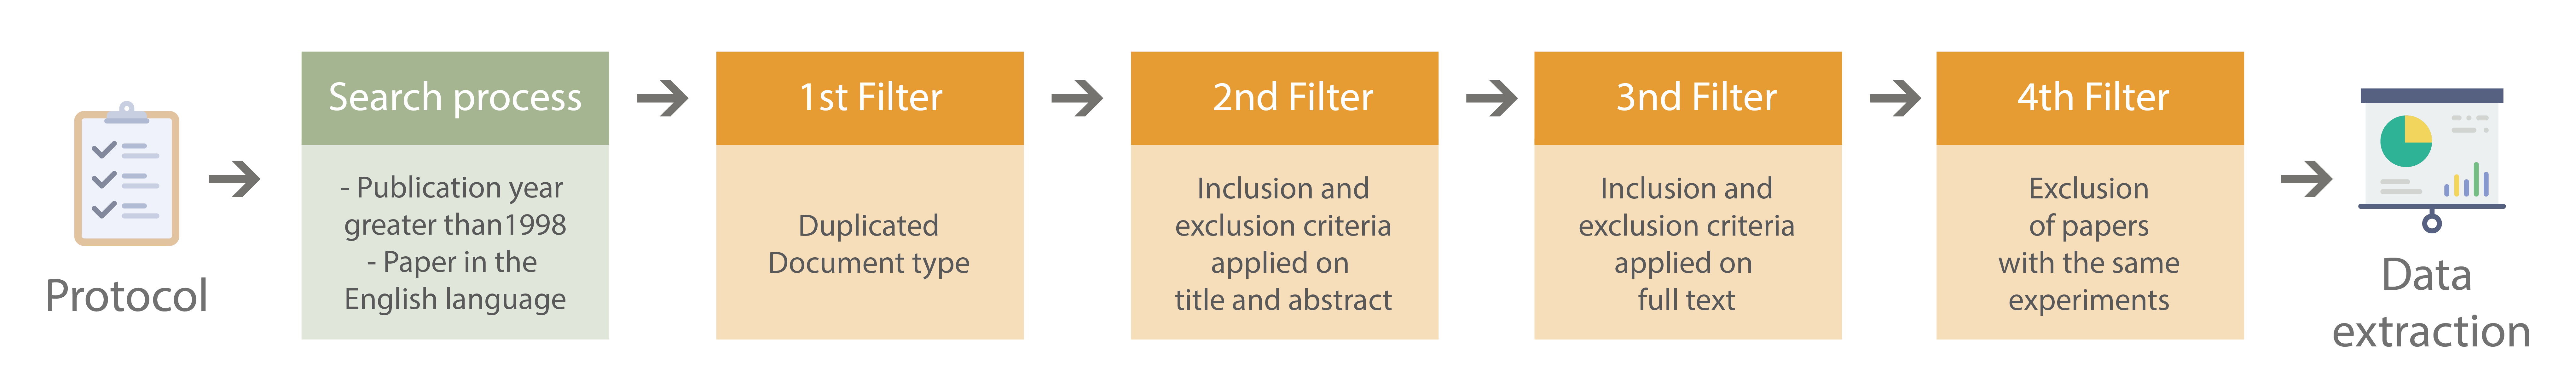
\includegraphics[width=16cm]{figuras/filters.png}
		}{
			\Fonte{Produced by the author.}
		}	
	\end{figure}
	
The first filter excluded papers duplicated and document types out the scope due their format (\textit{E.03}). The second filter identifies which paper is in and out the scope by reading their titles and abstracts (\textit{E.01}). A lot of papers were excluded in the first filter because the scientific base PubMed Central (PMC) brings a lot of medical papers focused on disease effectiveness and specific medical statements. Even though the area of this study is computer science, we decided to insert the PMC in the bases’ list due to the nature of the subject. 

Next, in the third filter, we evaluated each retrieved paper in its entirety (\textit{E.02}). If necessary, besides the entire text, we search more about the technologies and processes described, as project and institutional websites, videos, newspaper articles and others. In the fourth filter, we search and compare the experiments to find the same experiment described in two or more papers. This occurs when the experiment is not the primary goal of the paper, and more than one paper cites the experiment methodology and results according to the paper goal.

Once we have chosen the select papers, we extract all data required to achieve the objective. The organization of the data generates data synthesis, which will be shown in the Section \ref{sec:results-empirical}. The main reason for withdrawing papers in the last filter was the evaluation performed is out the search and at most times related to the system performance, e.g., sensor performance evaluation. 

In face the final papers selected, we make a snowballing approach for an opportunistic search for other relevant papers. Snowballing is a manual search using the reference and citations (known as backward and forward snowballing) list of a paper or the citations to the paper select aiming to identify additional papers \cite{Wohlin2014}. Thus, we perform other interaction among the forward and backward snowballing list to select the papers reading the title firstly and abstract and after the whole text. The only interaction of both snowballing processes is due to the resource limitation and the number of papers excluded in the first filter of these papers, that eliminates duplicated papers and unwanted document types.


In the snowballing process, the acceptance rate was high compared to the mainstream search. This acceptance rate is due to the purchased papers are closely related to the theme of tools for people who are blind and usually use similar processes of validation building.


% \subsubsection{Cross-validation}
% \label{subsubsec:methodology-cross-validation}

% The cross-validation process is used to create a protection mechanism to reduce the bias \cite{Kitchenham2007}. We invited 5 specialists on systematic literature reviews and software engineering and asked them to validate a sort of 10 papers among 20 offered, which we choose randomly from 195 papers selected in the second filter. We use their selection result to compare with our and to get the accuracy of the filter. 

% In this cross-validation, we are testing the third filter of the systematic literature review, on which we read the entire papers to select them regarding the inclusion criteria. For this reason, the form does not take account in exclusion criteria, and it takes only on inclusion criteria. Figure \ref{fig:cross_validation} shows the cover of cross-validation form which is available online\footnote{\url{https://lana184.typeform.com/to/Y604av}}.

%  	\begin{figure}[h] 
%   	    \captionsetup{width=14cm}%Da mesma largura que a figura
% 		\Caption{\label{fig:cross_validation} Cross-validation form}
% 		\UFCfig{}{
% 			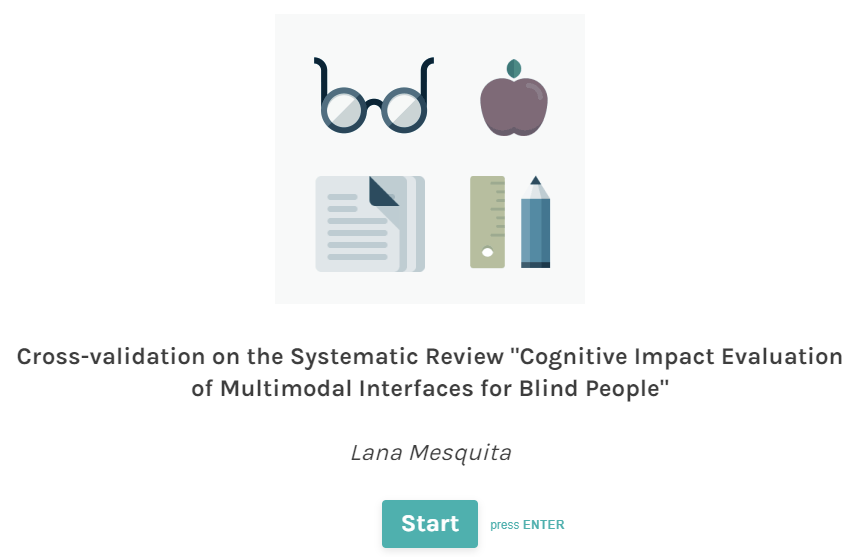
\includegraphics[width=14cm]{figuras/cross_validation.png}
% 		}{
% 			\Fonte{Produced by the author.}
% 		}	
% 	\end{figure}


\subsubsection{Studies quality evaluation}
\label{subsubsec:conducting-quality}

The quality evaluation for each paper accepted was based on the quality assessment in Table \ref{tab:quality_question} from \citeonline{Santos2017a}. Although the areas are different, the adaptations resulted in the following quality checklist to assess the studies and measure the weight of each study found on the results.

\begin{table}[h]
	\captionsetup{width=16cm}%Deixe da mesma largura que a tabela
	\Caption{\label{tab:quality_question} Quality assessment form}%
	\IBGEtab{}{%
		\begin{tabular}{m{1cm}m{14cm}}
			\toprule
			 & Quality Question \\
			\midrule \midrule
			\textbf{Q1} & Was it possible to extract all data regarding the data the Key features in multimodal interfaces (-0.1 pt per missing input; min value: -4.1 pts) \\
			\textbf{Q2} & Is there a complete description of how the evaluation has been applied? (1.0 pt per complete input in Empirical category; max value: 8,0 pts) \\
			\textbf{Q3} & Are the groups of participants in the experiment randomly assigned? (0.5 pt) \\
			\textbf{Q4} & Is the description of the impact evaluation understandable? (0.5 pt) \\
			\textbf{Q5} & Does the article present different evaluation types of the proposal? (1 pt) \\ 
			\textbf{Q6} & How many experiments does the paper present? (0.5 pt per experiment, if more than two experiments) \\
			\textbf{Q7} & Is the goal of the evaluation cleared defined? (0.5 pt) \\
			\textbf{Q8} & Is the hypothesis (null and alternative) explicitly described in the study? (0,5 pt) \\
			\bottomrule
		\end{tabular}%
	}{%
	\Fonte{Based on \citeonline{Santos2017a}.}%
%	\Nota{esta é uma nota, que diz que os dados são baseados na	regressão linear.}%
%	\Nota[Anotações]{uma anotação adicional, seguida de várias outras.}%
    }
    \end{table}

\subsubsection{Data Extraction Form Fields}
\label{subsubsec:methodology-data-extraction}

The data extraction was designed to answer the main and second questions and to understand the context in which each paper is inserted. We divide the data collected into three categories: \textit{(i)} General, \textit{(ii)} Research and \textit{(iii)} Empirical. The general category comprises bibliographic information. Table \ref{tab:data_collected} shows the data extracted and the categories.

\begin{table}[h]
	\captionsetup{width=13.2cm}%Deixe da mesma largura que a tabela
	\Caption{\label{tab:data_collected} Form for data collection}%
	\IBGEtab{}{%
		\begin{tabular}{m{1.2cm}m{10cm}m{1cm}}
			\toprule
			Category & Attribute & Type \\
			\midrule \midrule
			\multirow{7}{5em}{General} & Title & Text \\
			& The author(s) and affiliation & Text \\
			& The paper was published in a Journal, a Conference or as a Book chapter? & List \\
			& Year of publication & Number \\
			& Research type & List \\ 
			& Empirical Methods classification & List \\
			& Technologies the paper presents for people who are blind & Text \\ \hline
			\multirow{2}{5em}{Research} & Key features in multimodal interface & Text \\
			& Other strategies used to evaluate the interface (e.g. usability evaluation) & Text \\ \hline
			\multirow{8}{5em}{Empirical} & Sample & Text\\
			& Instruments & Text\\
			& Variables in the experimental design & Text\\
			& Statistical methods used & Text\\
			& Tasks defined & Text\\
			& Investigation cost (resources as time) & Text\\
			& Ethical concepts treated & Text\\
			\bottomrule
		\end{tabular}%
	}{%
	\Fonte{Produced by the author.}%
%	\Nota{esta é uma nota, que diz que os dados são baseados na	regressão linear.}%
%	\Nota[Anotações]{uma anotação adicional, seguida de várias outras.}%
    }
    \end{table}

The general category comprises bibliographic information and classifies the papers. We classified the  experiment of a scientific paper into two classifications: research type (Table \ref{tab:research_type_facet}), based on \citeonline{Petersen2008}. The research type is based on \citeauthor{Petersen2008} (\citeyear{Petersen2008}), which can be validation research, evaluation research, solution research, philosophical research, opinion paper or experience papers. The empirical method classification (Table \ref{tab:empirical__methods}) is based on the classification of \cite{Ampatzoglou2010}. This classification aims to confirm the papers retrieved are in the search focus, since we look for papers in the ``evaluation research'' type and that are ``Experiments''. Although, we retrieved one paper as a Case Study. For this one, we consider only the experiment data. All papers retrieved are in Evaluation Research category. 

\begin{table}[h]
	\captionsetup{width=16cm}%Deixe da mesma largura que a tabela
	\Caption{\label{tab:research_type_facet} Research type facet}%
	\IBGEtab{}{%
		\begin{tabular}{m{3cm}m{12cm}}
			\toprule
			Category & Description \\
			\midrule \midrule
			Validation Research & Techniques investigated are novel and have not yet been implemented in practice. Techniques used are for example experiments, i.e., work done in the lab. \\
			Evaluation Research & Techniques are implemented in practice and an evaluation of the technique is conducted. That means, it is shown how the technique is implemented in practice (solution implementation) and what are the consequences of the implementation in terms of benefits and drawbacks (implementation evaluation). This also includes to identify problems in industry. \\
			Solution Proposal & A solution for a problem is proposed, the solution can be either novel or a significant extension of an existing technique. The potential benefits and the applicability of the solution is shown by a small example or good line of argumentation. \\
			Philosophical Papers & These papers sketch a new way of looking at existing things by structuring the field in form of a taxonomy or conceptual framework. \\
			Opinion Papers & These papers express the personal opinion of somebody whether a certain technique is good or bad, or how things should been done. They do not rely on related work and research methodologies. \\ 
			Experience Papers & Experience papers explain on what and how something has been done in practice. It has to be the personal experience of the author. \\			\bottomrule
		\end{tabular}%
	}{%
	\Fonte{\citeonline{Petersen2008}.}%
%	\Nota{esta é uma nota, que diz que os dados são baseados na	regressão linear.}%
%	\Nota[Anotações]{uma anotação adicional, seguida de várias outras.}%
    }
    \end{table}
%%%Figura excluídda e comentada %%%
\begin{comment}
 	\begin{figure}[h] 
   	    \captionsetup{width=16cm}%Da mesma largura que a figura
		\Caption{\label{fig:research_type_facet} Research type facet}
		\UFCfig{}{
			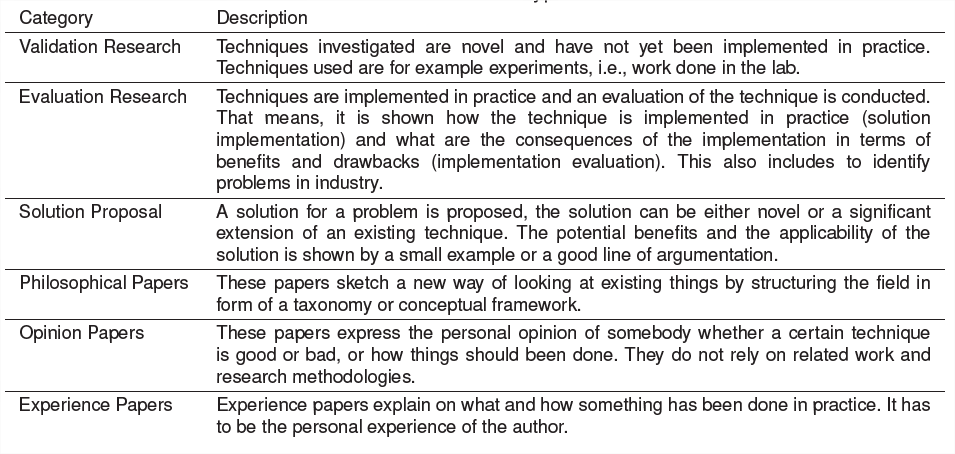
\includegraphics[width=16cm]{figuras/research_type_facet.png}
		}{
			\Fonte{\citeonline{Petersen2008}.}
		}	
	\end{figure}
\end{comment}

\begin{table}[h]
	\captionsetup{width=16cm}%Deixe da mesma largura que a tabela
	\Caption{\label{tab:empirical__methods} Empirical methods}%
	\IBGEtab{}{%
		\begin{tabular}{m{3cm}m{12cm}}
			\toprule
			Empirical method & Description \\
			\midrule \midrule
			Experiment & A set of a subjects is asked to perform a task in a highly controlled environment. the results are derived from observing of the subjects during the experiment, from inspecting the task outcome or from questioning the subjects at the end of the procedure.\\
			Survey & A set of subjects is asked to fill-in questionnaires either directly, or via internet. The results are derived from the valid answers to the questionnaire. \\
			Case study & A project, an activity or an assignment is monitored with respect to the methodology under study. Results are directly derived from project measurements. \\  \bottomrule
		\end{tabular}%
	}{%
	\Fonte{\citeonline{Ampatzoglou2010}.}%
%	\Nota{esta é uma nota, que diz que os dados são baseados na	regressão linear.}%
%	\Nota[Anotações]{uma anotação adicional, seguida de várias outras.}%
    }
    \end{table}

%%%Figura excluídda e comentada %%%
\begin{comment}
 	\begin{figure}[h] 
   	    \captionsetup{width=16cm}%Da mesma largura que a figura
		\Caption{\label{fig:empirical__methods} Empirical methods}
		\UFCfig{}{
			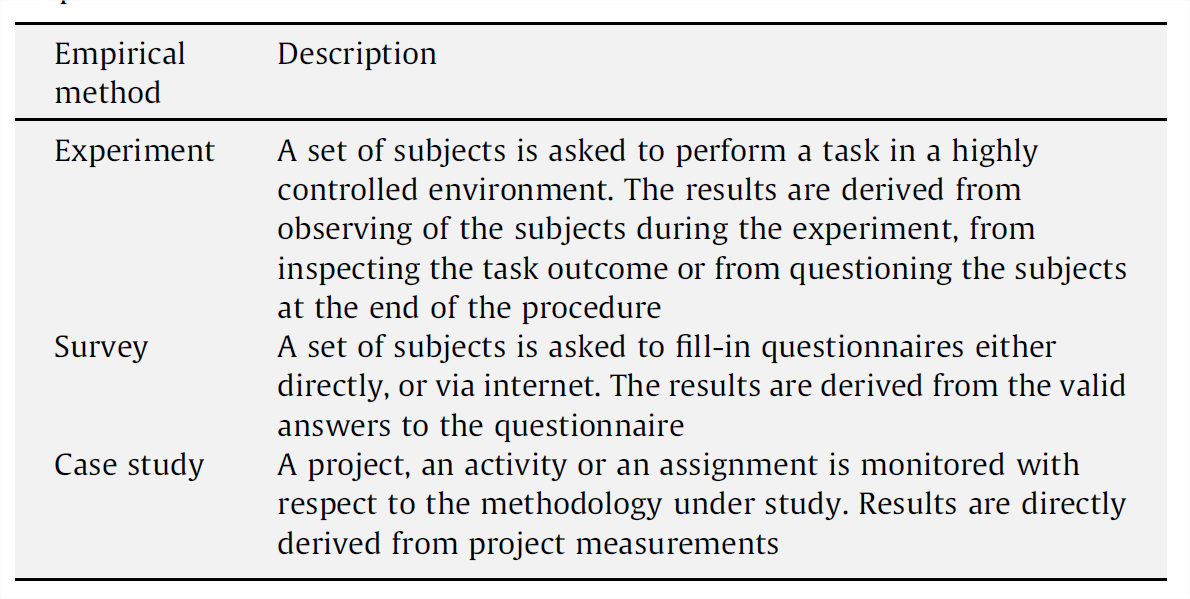
\includegraphics[width=16cm]{figuras/empirical__methods.png}
		}{
			\Fonte{ \citeonline{Ampatzoglou2010}.}
		}	
	\end{figure}
\end{comment}

The research category comprises the classification that fits the technology presented in the key features of multimodal interfaces for the cognition of people who are blind \cite{Darin2015}. This classification is divided into 4-dimension: Interface, Interaction, Cognition, and Evaluation; and it is applied to video games and virtual environments (Figure \ref{fig:key_features_multimodal_interfaces}).

 	\begin{figure}[h] 
   	    \captionsetup{width=14cm}%Da mesma largura que a figura
		\Caption{\label{fig:key_features_multimodal_interfaces} Key features in multimodal interfaces}
		\UFCfig{}{
			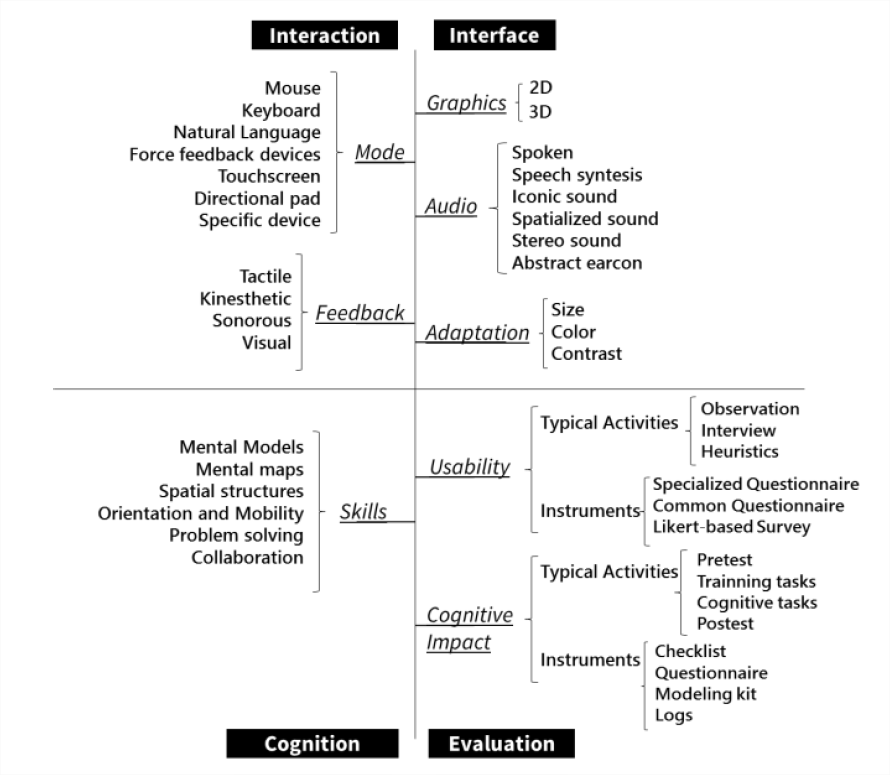
\includegraphics[width=14cm]{figuras/key_features_multimodal_interfaces.png}
		}{
			\Fonte{ \citeonline{Darin2015}.}
		}	
	\end{figure}

For our purpose, we classify only in the interaction, interface and cognition dimensions; and we cover, in the classification, more than video games and virtual environments, since we also found these features present in the technologies selected. These features provide necessary insights for the practical understanding of the issues involved in their design and evaluation \cite{Darin2015}. They are useful in our research for giving a comprehensive overview of technologies and evaluations regarding the multimodal interfaces. The research category still shows more information about the research, as other strategies used to evaluate.

The empirical category provides information specifically about how the empirical method that evaluates the impact of the cognitive impact. These data are more explained in the Results chapter (Section \ref{chap:resultados}).

\section{Grounded Theory}
\label{sec:methodology-gt}

The Grounded Theory, introduced by Barney Glaser and Anselm Strauss, is a method at the beginning used on health studies \cite{Glaser1967}. \citeonline{Glaser1967} contrast theory generated by deduction and a priori assumptions with the theory discovery arising from and grounded in research data, through constant comparison. ``One can argue that every research is somehow "grounded" in data, but using this data from systematic research, together with a set of rigorous research procedures to produce a "grounded theory" is a different approach'' \cite{Motta2016}. The employee of the Grounded Theory method is recent in Empirical Software Engineering. 

The Grounded Theory analysis was performed to enhance and strengthen the findings of the Systematic Literature Review regarding cognitive evaluation concepts used in the context of this search, multimodal interfaces for people who are blind. The data gathered from the literature become the population used in the analysis. We aim analyze in the deepest level of generating theory but as the authors state: knowledge and understanding take many forms \cite{Corbin1998}. The Grounded Theory was supported by the MAXQDA12\footnote{MAXQDA - \url{https://www.maxqda.com/}} tool in the whole process, which is composed of the following steps: planning, data collection, coding and reporting results.

The planning step aims to identify the area of interest and the research question that drives the work. In our case, the area of interest is the Cognitive Impact Evaluation. In the current research, the Grounded Theory suits well some characteristics of cognitive impact experiment extracted from the systematic review as it aids in the interpretation and clarification of the results found. The Grounded Theory methodology comes as a mechanism to understand this data and how they relate to each other considering the application domain and evaluation features.


%%%%Refazer imagem com termos utilizados e sequencia.%%%%

% 	\begin{figure}[h] 
%   	    \captionsetup{width=16cm}%Da mesma largura que a figura
% 		\Caption{\label{fig:grounded_theory__process} Grounded Theory process}
% 		\UFCfig{}{
% 			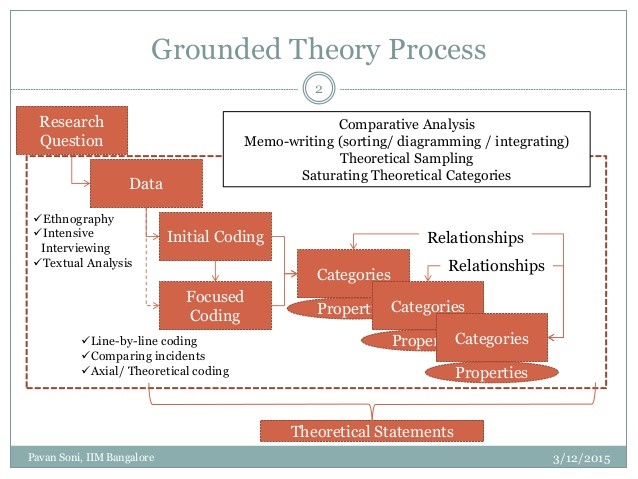
\includegraphics[width=16cm]{figuras/grounded_theory__process.jpg}
% 		}{
% 			\Fonte{ \citeonline{Charmaz2006}.}
% 		}	
% 	\end{figure}

In the data collection step, we prepare an Excel spreadsheet with data from the Systematic Literature Review. We import the data extraction form from each experiment into the MAXQDA. In this way, each experiment is a document in the MAXQDA analysis. All data from experiments are imported as variables (59 variables), that could be used to quantify your qualitative analysis results or to add additional information to pieces of data. These one are already imported as excerpts coded as the empirical categories. 

The data retrieved is organized and modified from the paper to answer the data form. Although, in some experiments, we add some excerpt from the paper to facilitate the coding step on that experiment.

The coding step, the heart of the Grounded Theory, is composed of (i) Open Coding, (ii) Axial Coding, and (iii) Selective Coding. On this step we extracted concepts from raw data and relate them to each other until reaching a core concept \cite{Wuetherick2010}. In our case, we envisioned and related some concepts of experiments of cognitive impact evaluation.

The excerpts coded in this step could be a word, a phrase or a full paragraph when relevant for the concept under observation at the moment. We explore the experiments and open up the data to all potentials and possibilities contained within them \cite{Wuetherick2010}. After considering all possible meanings and examining the context carefully produced 91 codes and 808 tags. Figure \ref{fig:open_coding} shows the 6 top categories of the codes. 

To uncover and develop the concepts one has to keep the mind open and also report thoughts and ideas related to it. The researcher scrutinizes the data in an attempt to understand the essence of what is being expressed in the raw data \cite{Wuetherick2010}. 

 	\begin{figure}[h] 
   	    \captionsetup{width=13cm}%Da mesma largura que a figura
		\Caption{\label{fig:open_coding} Open Coding}
		\UFCfig{}{
			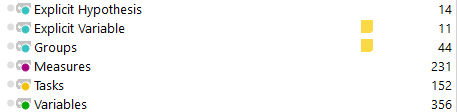
\includegraphics[width=13cm]{figuras/open_coding.png}
		}{
			\Fonte{Produced by the author.}
		}	
	\end{figure}

In the open coding, constant comparative analysis is a regular procedure to execute it. Whenever coming across another excerpt that seemed to talk about the same concept or shared a common attribute, these were grouped together into the same code. 

Axial Coding is stepping to relate concepts to each other \cite{Wuetherick2010}. With this step, the fractions of data from the open coding can be reassembled and organized into the categories and subcategories with their descriptions, properties or dimensions. The Axial Code produced 95 codes and 603 tags. 

The Selective Coding merge all concepts grounded in the process and others captured in the Systematic Literature Review. As a result, we produce maps of concepts and a map to ground the theory of the cognitive impact evaluation in multimodal interfaces for people who are blind or visually impaired. All maps are presented in the chapter Results (Section \ref{chap:resultados}). 
